\documentclass[12pt, titlepage]{article}

\usepackage{booktabs}
\usepackage{tabularx}
\usepackage{hyperref}
\hypersetup{
    colorlinks,
    citecolor=black,
    filecolor=black,
    linkcolor=red,
    urlcolor=blue
}
\usepackage[round]{natbib}
\usepackage{float}
\usepackage{graphicx} 
\usepackage{array}
\usepackage{booktabs} 
\usepackage{longtable}

%% Comments

\usepackage{color}

\newif\ifcomments\commentstrue %displays comments
%\newif\ifcomments\commentsfalse %so that comments do not display

\ifcomments
\newcommand{\authornote}[3]{\textcolor{#1}{[#3 ---#2]}}
\newcommand{\todo}[1]{\textcolor{red}{[TODO: #1]}}
\else
\newcommand{\authornote}[3]{}
\newcommand{\todo}[1]{}
\fi

\newcommand{\wss}[1]{\authornote{blue}{SS}{#1}} 
\newcommand{\plt}[1]{\authornote{magenta}{TPLT}{#1}} %For explanation of the template
\newcommand{\an}[1]{\authornote{cyan}{Author}{#1}}

%% Common Parts

\newcommand{\progname}{PCD: Partially Covered Detection of Obscured People using Point Cloud Data} % PUT YOUR PROGRAM NAME HERE
\newcommand{\authname}{Team \#14, PCD
\\ Tarnveer Takhtar
\\ Matthew Bradbury
\\ Harman Bassi
\\ Kyen So} % AUTHOR NAMES                  

\usepackage{hyperref}
    \hypersetup{colorlinks=true, linkcolor=blue, citecolor=blue, filecolor=blue,
                urlcolor=blue, unicode=false}
    \urlstyle{same}

\usepackage{indentfirst}                              


\begin{document}

\title{Verification and Validation Report: \progname} 
\author{\authname}
\date{\today}
	
\maketitle

\pagenumbering{roman}

\section{Revision History}

\begin{tabularx}{\textwidth}{p{3cm}p{2cm}X}
\toprule {\bf Date} & {\bf Version} & {\bf Notes}\\
\midrule
Date 1 & 1.0 & Notes\\
Date 2 & 1.1 & Notes\\
\bottomrule
\end{tabularx}

~\newpage

\section{Symbols, Abbreviations and Acronyms}

\renewcommand{\arraystretch}{1.2}
\begin{tabular}{l l} 
  \toprule		
  \textbf{symbol} & \textbf{description}\\
  \midrule 
  T & Test\\
  \bottomrule
\end{tabular}\\

\wss{symbols, abbreviations or acronyms -- you can reference the SRS tables if needed}

\newpage

\tableofcontents

\listoftables %if appropriate

\listoffigures %if appropriate

\newpage

\pagenumbering{arabic}

This document outlines the results and analysis of executing our VnV plan. Included below is a brief summary of each Functional, Non-functional, and Unit test, along with a description of their expected vs actual results. Provided with these results is the insight gained on the system that each tests highlights. "N/I" will be used for tests that have not yet been implemented.  

\section{Functional Requirements Evaluation}

\subsection{Human Detection Testing}
The following section covers the functional tests related to human detection given different coverage levels.

\subsection{Offline Processing}
The following section covers the functional tests related to the offline processing of files.

\subsection{Body Pose Variation Handling}
The following section covers the functional tests related to human detection give a dynamic set of poses.

\subsection{Integration with Kinect Sensor}
The following section covers the functional tests related to the connection and data transfer of the Kinect Sensor.

\subsection{Location Prediction Test}
The following section covers the functional tests related to predicting the location of obscured segments.

\section{Non-Functional Requirements Evaluation}

\subsection{Realtime Processing}
The following section covers the non-functional tests related to performance metrics.
		
\subsection{Reliability}
The following section covers the non-functional tests related to reliability requirements.

\subsection{Accuracy}
The following section covers the non-functional tests related to accuracy requirements.

\section{Unit Testing}

\begin{table}[H] % Force table to stay here
  \centering
  \renewcommand{\arraystretch}{1.4} % Adjust row height for better readability
  \resizebox{\textwidth}{!}{ % Ensures table fits within text width
  \begin{tabular}{|p{1.5cm}|p{2.5cm}|p{3cm}|p{4cm}|p{4cm}|p{1.8cm}|}
      \hline
      \textbf{ID} & \textbf{Type} & \textbf{Input} & \textbf{Expected Result} & \textbf{Actual Result} & \textbf{Pass/Fail} \\
      \hline
      UT1 & Automated & \raggedright Sample PCL Point Cloud \par & \raggedright The RGB values, Depth Values, and Cloud Size are mapped correctly between file types. \par & \raggedright The RGB values, Depth Values, and Cloud Size are mapped correctly between file types. \par & Pass \\
      \hline
      \multicolumn{6}{|p{\textwidth}|}{\raggedright \textbf{Description:} ConvertPCLtoOpenCV: Converts a PCL Point Cloud to OpenCV Mat type for point cloud analysis using OpenCV. A pass means that the function correctly maps the Point Cloud values to OpenCV Mat type. The unit test passed successfully, verifying that the mapped values matched between the two types. \par} \\
      \hline
      UT2 & Automated & \raggedright OpenCV Mat, Min Depth, Max Depth \par & \raggedright Returns an OpenCV Mat Type that includes only points within the desired depth range. \par & \raggedright Returns an OpenCV Mat Type that includes only points within the desired depth range. \par & Pass \\
      \hline
      \multicolumn{6}{|p{\textwidth}|}{\raggedright \textbf{Description:} segmentDepth: This function takes an OpenCV Mat cloud and removes points outside the specified depth range. A pass indicates that only points within the given depth range remain in the returned Mat. The unit test passed, confirming correct depth segmentation. \par} \\
      \hline
  \end{tabular}
  }
\end{table}


\section{Changes Due to Testing}

\wss{This section should highlight how feedback from the users and from 
the supervisor (when one exists) shaped the final product.  In particular 
the feedback from the Rev 0 demo to the supervisor (or to potential users) 
should be highlighted.}

\section{Automated Testing}

The only automated testing present is the Unit Tests, which are run using CTest and GTest Suites.
		
\section{Trace to Requirements and Modules}		
See section G.4 in the \href{https://github.com/takhtart/PCD/blob/main/docs/SRS/SRS.pdf}{SRS report} for more information on the requirements. See section 7 in the \href{https://github.com/takhtart/PCD/blob/main/docs/Design/SoftArchitecture/MG.pdf}{Module Guide} for more information on the modules.

\begin{table}[H]

  \centering
  \caption{Module and Requirement Tracing}
  \begin{tabular}{|l|l|l|}
  \hline
  \textbf{Test ID} & \textbf{Requirement ID} & \textbf{Modules}\\
  \hline
  FT11 & F411 & M5, M6, M7, M8, M9\\
  \hline
  FT12 & F411 & M5, M6, M7, M8, M9\\
  \hline
  FT13 & F411 & M5, M6, M7, M8, M9\\
  \hline
  FT14 & F411 & M5, M6, M7, M8, M9\\
  \hline
  FT15 & F411 & M5, M6, M7, M8, M9\\
  \hline
  FT16 & F411 & M5, M6, M7, M8, M9\\
  \hline
  FT17 & F411 & M5, M6, M7, M8, M9\\
  \hline
  FT18 & F411 & M5, M6, M7, M8, M9\\
  \hline
  FT21 & F412 & M7, M11\\
  \hline
  FT22 & F412 & M7, M11\\
  \hline
  FT23& F412 & M7, M11\\
  \hline
  FT24 & F412 & M7, M11\\
  \hline
  FT31 & F413 & M4, M5, M6, M8, M9, M10, M11\\
  \hline
  FT32 & F413 & M4, M5, M6, M8, M9, M10, M11\\
  \hline
  FT41 & F414 & M4, M5, M6, M8, M9\\
  \hline
  FT42 & F414 & M4, M5, M6, M8, M9\\
  \hline
  FT43 & F414 & M4, M5, M6, M8, M9\\
  \hline
  FT51 & F415 & M1, M2\\
  \hline
  FT52 & F415 & M1, M2\\
  \hline
  NFT11 & NF431 & M1, M2, M9\\
  \hline
  NFT12 & NF432 & M5, M6, M7, M9\\
  \hline
  NFT13 & NF433 & M5, M6, M7\\
  \hline
  \end{tabular}
\end{table}

\section{Code Coverage Metrics}

The automated unit testing achieves 6\% line coverage. This is checked using CTest and OpenCPPCoverage Suites to acquire coverage results.\\
\\
OpenCPPCoverage Result:

\begin{figure}[h]
    \centering
    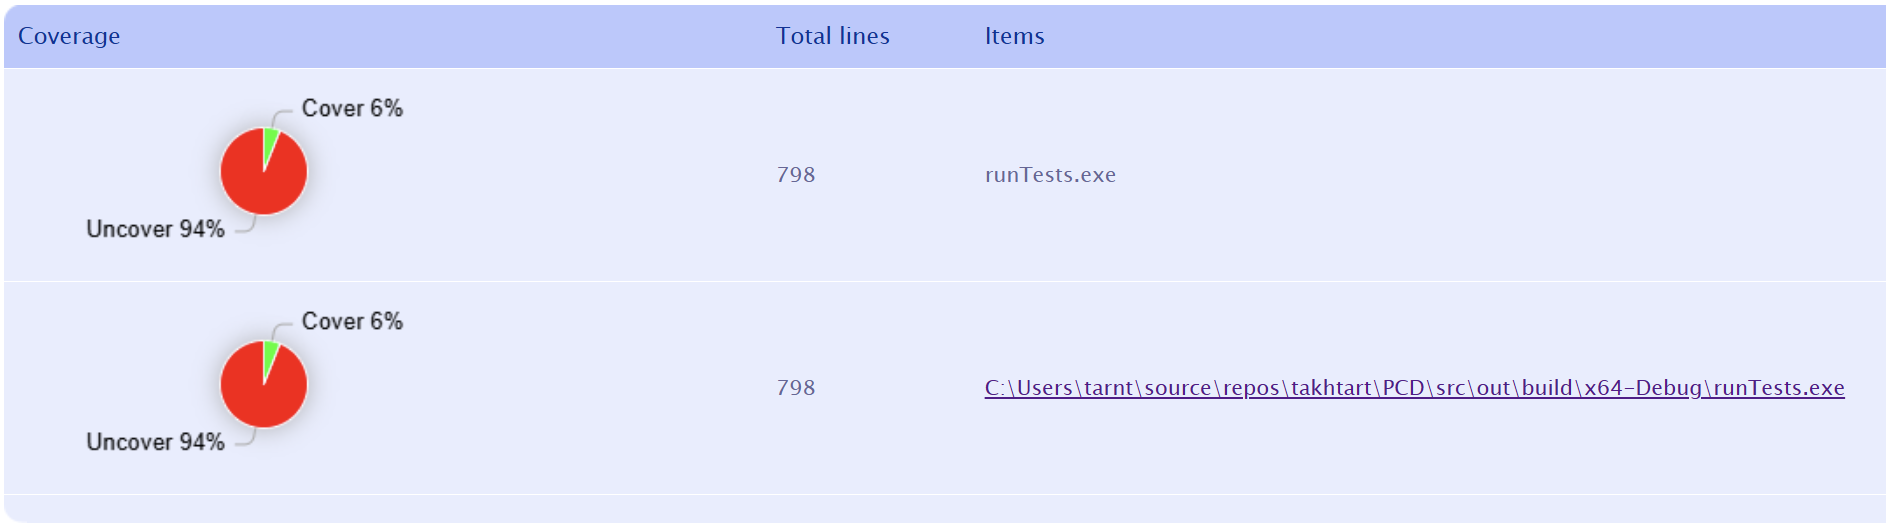
\includegraphics[width=1\textwidth]{Coverage.png} % Adjust width as needed
    \caption{OpenCPPCoverage Result}
    \label{fig:coverage}
\end{figure}

\bibliographystyle{plainnat}
\bibliography{../../refs/References}

\newpage{}
\section*{Appendix --- Reflection}

The information in this section will be used to evaluate the team members on the
graduate attribute of Reflection.

\begin{enumerate}
  \item What went well while writing this deliverable? \\
  \\
  When writing this deliverable, the sections that were very smooth were the ones that stemmed directly from the VnV plan. Those sections that went exactly as planned as the VnV Plan were very easy to translate to this report.
  \item What pain points did you experience during this deliverable, and how
    did you resolve them? \\
  \\
  A slight pain point that we did run into had to do with a change we received from Dr. Bone after Rev0. He proposed a change clarifying his vision for the project. This change caused one of our requirements to be completely reworked, changing the associated tests as well. We resolved this by simply moving back and rewriting the requirement, planned tests, and report tests that related to this requirement.
  \item Which parts of this document stemmed from speaking to your client(s) or
  a proxy (e.g. your peers)? Which ones were not, and why?\\
  \\
  The parts of the document that stemmed from speaking to our supervisor were the ones relating to the requirement mentioned in the above question. The rest of the requirements we generated previously based on the initial specification from Dr. Bone, which he checked and approved. The only new tests, that weren't described in the VnV Plan, were those related to the new reworked requirement stemming from Dr. Bone's feedback.
  \item In what ways was the Verification and Validation (VnV) Plan different
  from the activities that were actually conducted for VnV?  If there were
  differences, what changes required the modification in the plan?  Why did
  these changes occur?  Would you be able to anticipate these changes in future
  projects?  If there weren't any differences, how was your team able to clearly
  predict a feasible amount of effort and the right tasks needed to build the
  evidence that demonstrates the required quality?  (It is expected that most
  teams will have had to deviate from their original VnV Plan.) \\
  \\
  Aside from the changes mentioned in the previous question, we had to slightly tweak some of the test procedures initially proposed in the VnV Plan. In the beginning we weren't set on what method we were using for human detection and ended up trying a few different ways. The test procedures were initially written without any specific method in mind. Later on, after many meetings with Dr. Bone, we settled on a method that mainly uses skin point detection and region growing. Because of this method some of the test procedures didn't really make sense, namely any one that caused the person to maneuver into a position that hid all skin from the camera. The changes that this required was simply to move back to the VnV plan and tweak the procedure in such a way that kept the original intent of the test but made it feasible to test with our method of detection. Regarding these issues, I don't think we would be able to predict roadblocks like this in the future. The nature of these issues stem from explorations during development and would be difficult to account for prior.
\end{enumerate}

\end{document}